


%\section{Associativity in Virtual Memory}
\section{SpryVM: Hardware Support}
\label{sec:associativity}

%\javier{ Points to come across:
%
%\begin{itemize}
%  \item We can have a first subsection to talk about the 4 points of the intro's table (i.e., programmability, power/perf, flexibility, safety). What we would like to have, the goal. 
%  \item We can have second subsection to talk about the problems of full associativity, and the idea of set associativity, which is essentially partitioning the memory and translation information and knowing to which memory set to go, and how that can help at the aforesaid 4 points. We can have a high-level figure on how the memory and the translation information is partitioned. 
%  NOTE: This section has to be short, maximum one page, and zero results! It has to be high level!!!
%\end{itemize}

%}

We compare the hardware necessary for SpryVM with conventional
TLBs. We first walk the reader through a translation operation in a
conventional memory management mechanism and then we present the same
operation in SpryVM.

\subsection{Baseline Address Translation}

Figure \ref{fig:pagewalk_base} illustrates the timeline of
conventional address translation. In the conventional case, a TLB is
first probed by the acclerator it resides in. Consider the case of a
TLB miss on an accelerator without caches residing close to memory, as
considered in recent work \cite{haria:devirtualizing,
  picorel:near-memory}. The accelerator's hardware page table walker
identifies the physical address of the page table and initiates a
lookup of it. Page tables can be implemented in many ways, e.g., radix
tree, inverted, hashed, etc. Consider the scenario where either
because of the page table structure or the presence of MMU caches
\cite{bhattacharjee:large-reach, barr:translation}, the entire page
table walk amounts to a single memory reference lookup. This lookup
can result in a probe of any location in memory. Consequently, we may
need to traverse the NoC and off-chip interconnect to locate the
memory channel hosting the desired page table entry. Once the memory
channel is identified, its memory controller accesses the page table
entry's location in DRAM, and then page table entry, which holds the
virtual-to-physical translation information is found. The page table
entry has to return to the accelerator, again prompting NoC and
off-chip interconnect traversal. Once the page table entry is returned
to the accelerator, TLB fill occurs. This part of the timeline
constitutes th translation path.

Subsequently, the accelerator uses the page table entry to calculate
the physical address of the data fetch. A set of NoC and off-chip
interconnects are traversed to locate the memory channel that holds
the piece of data, and its memory controller access DRAM. Once the
memory controller receives the data, the data has to traverse the same
NoC and off-chip interconnects to return to the accelerator. This part
of the timeline constitutes the data fetch.

Figure \ref{fig:pagewalk_base} shows that conventional address
translation is expensive. First, the TLB's accelerator-side
integration means that it must address all of physical memory, which
can elevate its miss rate. Second, when these misses occur,
translation and data paths may not overlap. Hence, translation walk
latency is on the critical path of the memory access.


\subsection{SpryVM Address Translation}

In SpryVM, instead of integrating a TLB per accelerator, we integrate
a TLB per region of physical memory a virtual address is able to
uniquely identify. In our case, we restrict the associativity so that
each TLB is responsible to translating the virtual addresses mapped to
a memory channel (check Figure 1). Hence, each TLB is responsible of a
narrower part of the physical memory, increasing the hit rates of the
TLBs. Figure~\ref{fig:pagewalk_partition_hit} shows the timeline of
events when an accelerator issues a memory reference which hits in one
of SpryVM's TLBs. In SpryVM, as a virtual address uniquely identifies
a memory region, the virtual address is used as a memory request,
requiring traversing NoC and off-chip interconnect to locate the
appropriate memory channel. Then, a simple multiplexer (not shown in
the figure) distinguishes between virtual and physical address
requiests, and sends the aforesaid required to the memory channel's
TLB. The TLB holds the translation information and hence the page
frame and the physical address of the data is known. This set of
events constitute the translation path.

Now since the appropriate page table entry is in the TLB and the page frame is located in the memory channel, the data path begins by the memory controller accessing the DRAM arrays to fetch the data. Once the data returns to the memory controller, the data is sent back to the accelerator traversing the same NoC and off-ship interconnects. This set of events constitute the data path.

As shown in the figure, TLB hits completely overlap the translation with the data path, because the time to locate the memory channel takes part of both paths at the same time. Hence, the translation overhead is exactly zero, equal to an ideal translation mechanism. Furthermore, we make sure that TLB hits are more often than in the conventional translation as TLB are responsible of translation of a narrow part of the physical memory space.

Although SpryVM significantly reduce the frequency of TLB misses, page walks can still occur. Figure~\ref{fig:pagewalk_partition_miss} shows the timeline of events when an accelerator issues a memory reference that misses in one of SpryVM's TLBs. In such cases, and similar to the previous case, the virtual address is used to arrive at the appropriate memory controller traversing the NoC and off-chip interconnects. Then, upon a TLB miss, a page table, similarly to the TLBs, only responsible for holding page table entries that map to the region of physical memory, is referenced. Note that unlike in the conventional translation mechanism, there is no need to traverse the NoC and off-chip interconnects for the page walk operation. Once the page table entry arrives from the DRAM arrays and the TLB fill operation completes, the translation path finishes. Then, memory controller issues the complete physical address to locate the target piece of data. Then, when data returns from the DRAM array, it is sent back to the accelerator by traversing the networks, finishing the data path.

In this case, page walks are still much cheaper than in conventional translation as the time to locate the appropriate memory channel is part of both the translation path and data path, essentially removing this part of the cost of address translation. Furthermore, page walks do not further involve network communication as the page table entries are all locate in the same memory channel. Note that the larger the latency of the network is with respect to the DRAM accesses, the lower overhead of page walks in SpryVM. This behavior benefits large memory systems, as the need for scaling out the memory for large-memory machines increase the average distance to the memory channels. 


\begin{figure*}
	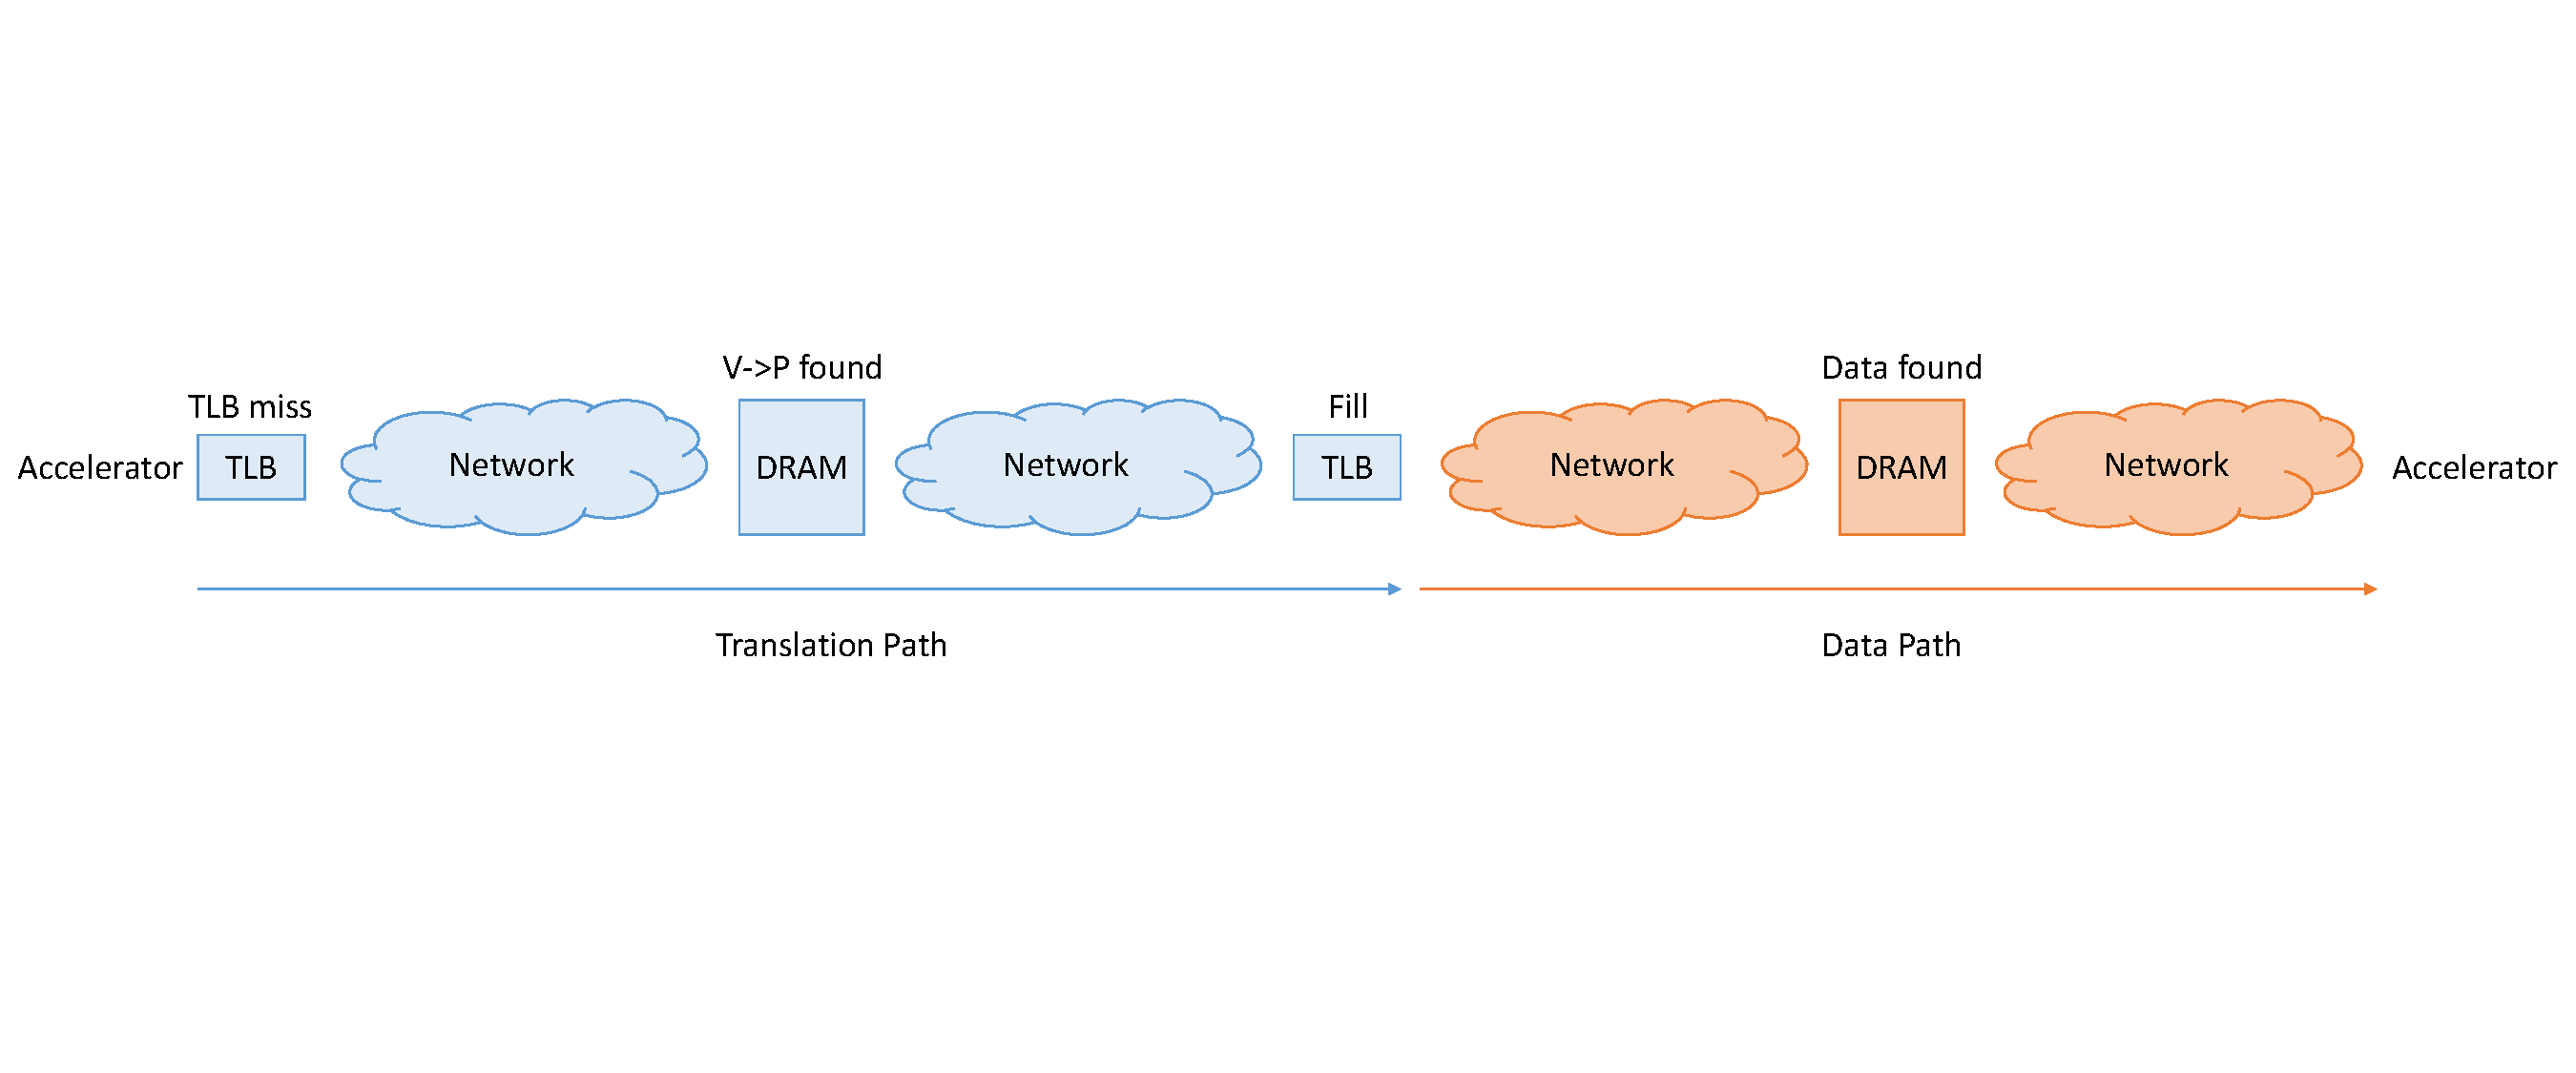
\includegraphics[width=\textwidth]{figures/time_event_base.pdf}
	\caption{Timeline of events of an accelerator's memory reference that misses in the TLB on conventional translation.}
	\label{fig:pagewalk_base}
\end{figure*}

\begin{figure*}
	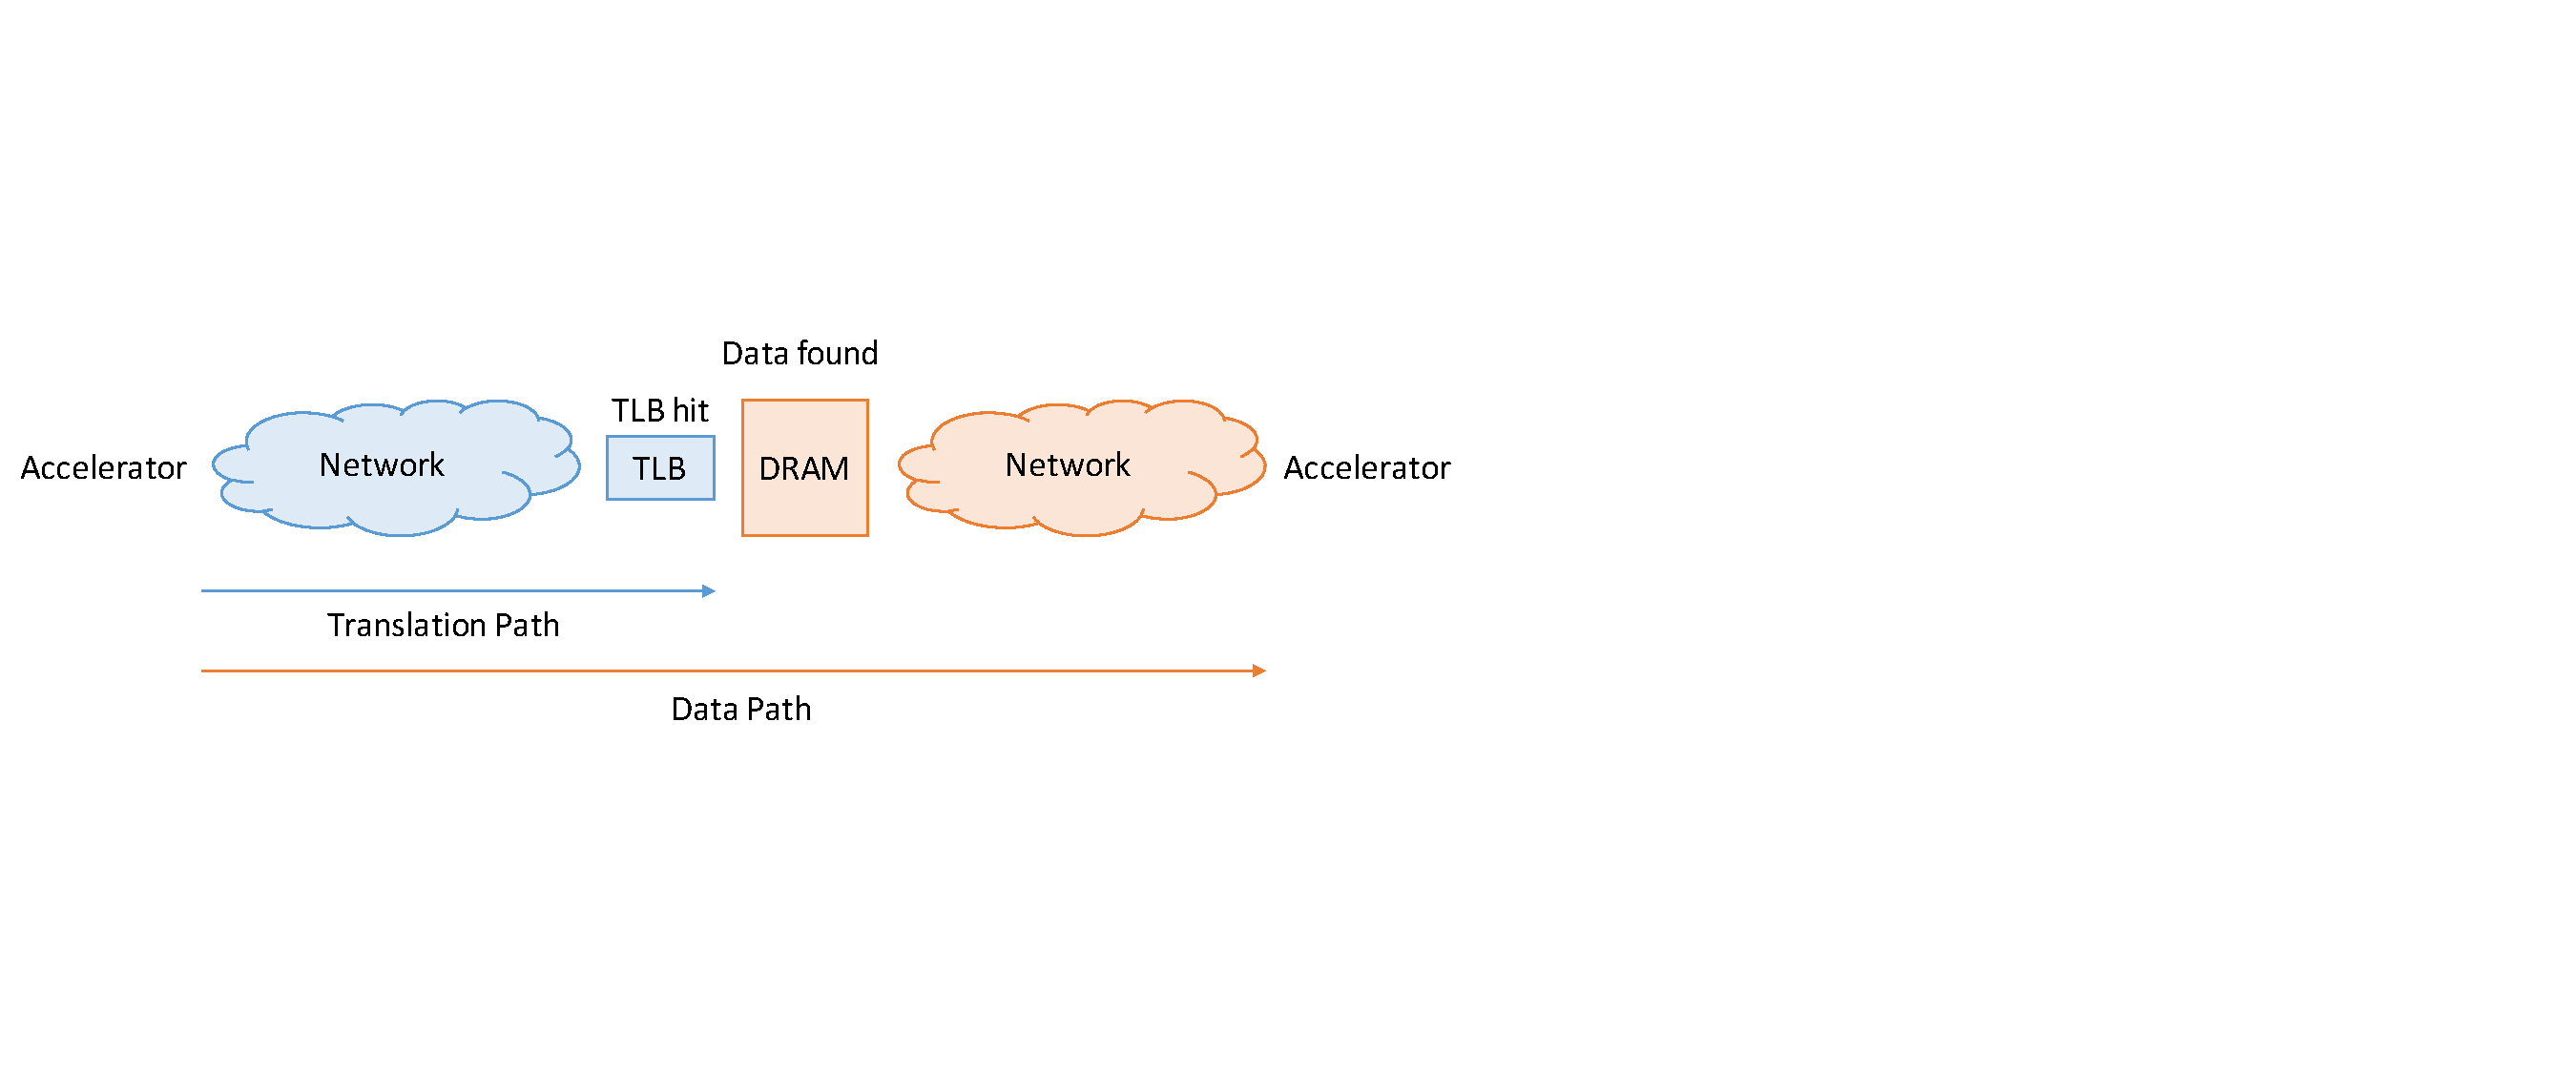
\includegraphics[width=\textwidth]{figures/time_event_partition_hit.pdf}
	\caption{Timeline of events of an accelerator's memory reference that hits in the TLB on SpryVM.}
	\label{fig:pagewalk_partition_hit}
\end{figure*}

\begin{figure*}
	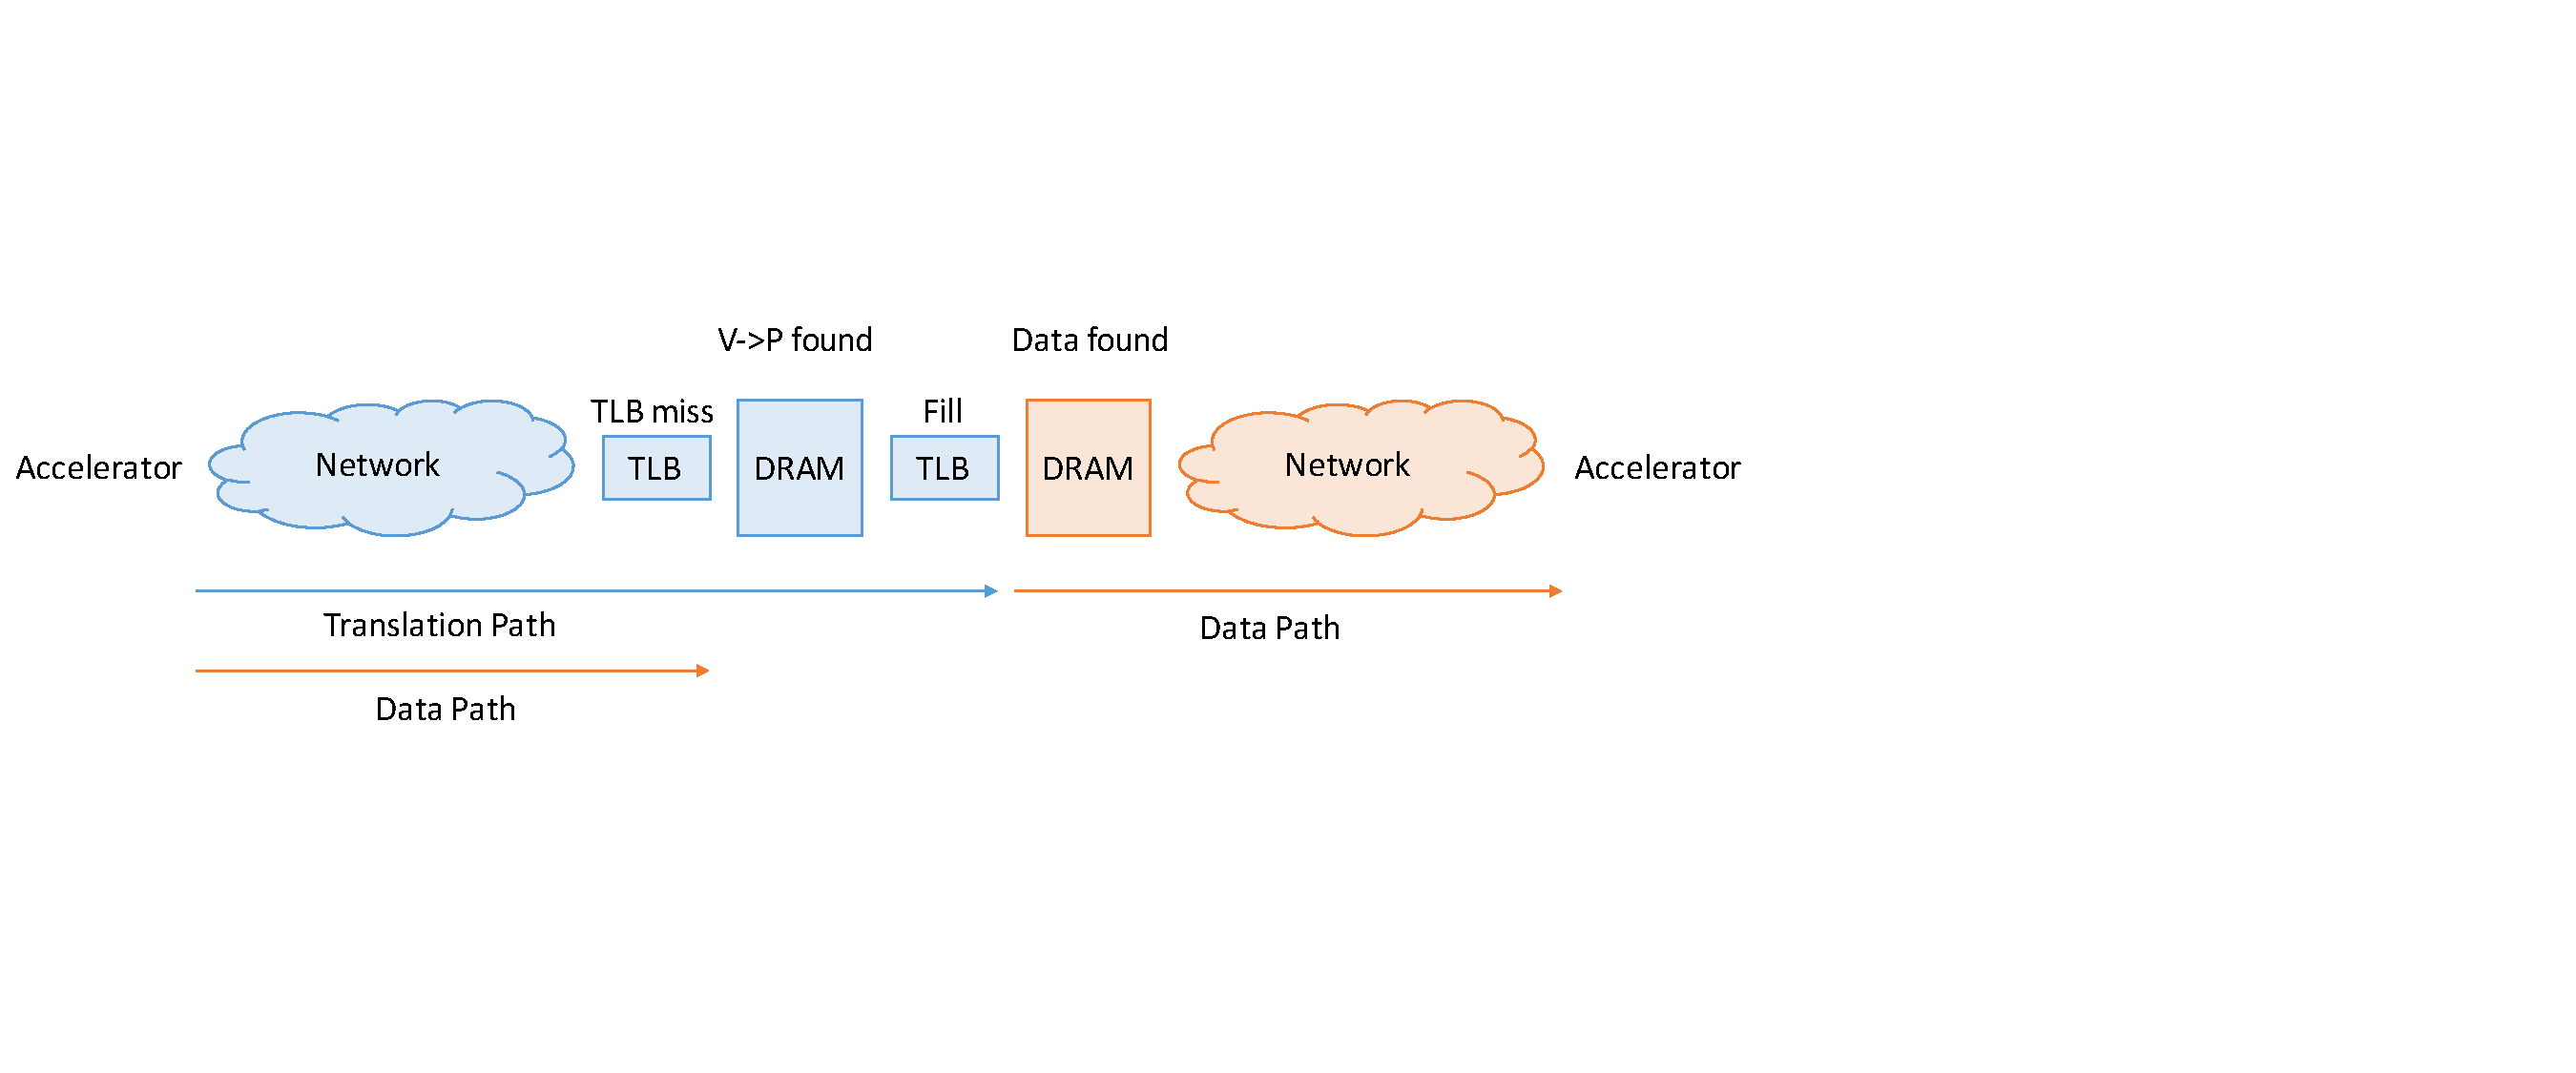
\includegraphics[width=\textwidth]{figures/time_event_partition_miss.pdf}
	\caption{Timeline of events of an accelerator's memory reference that misses in the TLB on SpryVM.}
	\label{fig:pagewalk_partition_miss}
\end{figure*}


 
%In modern page-based VM, a virtual page is mapped on demand into a page frame. Modern systems place no restrictions on the virtual-to-physical mapping; a virtual page can potentially map to any page frame. Though flexible, this fully associative approach places translation on the critical path of every memory access, because a memory access cannot begin until the translation operation finishes.

%One potential way to break translation-memory access serialization is to completely eliminate associativity and enforce a direct mapping between virtual pages and page frames. Since a virtual page can now only map to a single page frame, address translation and data fetch are independent and can proceed in parallel. Conventional wisdom dictates that direct mapping creates an excess of page faults, due to conflicts from multiple virtual pages mapping to the same page frame. However, this is merely intuition, as there exists no study on VM associativity, unlike caches, which are similar in some organizational aspects and for which such a study has existed for three decades~\cite{hill:aspects}. 



%To fill this research void, we employ the 3C model---initially developed for caches~\cite{hill:aspects}---to study VM associativity. In this context, associativity means the number of possible locations (page frames) a given virtual page can map to. This model classifies misses (i.e., page faults) into three categories: conflict misses (when too many active pages map to a fraction of the sets), capacity misses (due to limited memory size), and compulsory misses (upon the first access to a page). 

%To simulate real-world scenarios, we select a set of representative server workloads, summarized in Table~\ref{table:workload}. We include two cloud workloads from CloudSuite~\cite{ferdman:clearing}, Cassandra and Memcached, an online transaction processing (OLTP) workload~\cite{facebook:linkbench}, MySQL, two online analytical processing (OLAP) workloads~\cite{boncz:breaking}, TPC-H and TPC-DS, and a widely-used storage system workload~\cite{dong:optimizing}, RocksDB. We collect long memory traces of several 10s of billions of instructions of the server workloads using Pin~\cite{luk:pin}. We extract the virtual address and address space identifier (ASID) of each memory reference and use it to probe a set-associative memory structure, varying the associativity to observe and classify the misses. A detailed description of our methodology is found in Section~\ref{sec:methodology}.

%\subsection{Single-Process In-Memory}

%Fig.~\ref{fig:miss_ratio} shows results for three single-process workloads: Memcached, RocksDB, and Cassandra. The y-axis breaks down the total misses into the three distinct miss classes. Each category on the x-axis corresponds to the ratio between the size of the physical memory and the size of the application's working set. For example,  $8\times$ indicates that the memory is eight times larger than the application's working set. Similarly, $1/2\times$ means that the application's working set is twice the size of the memory. We collapse results for $8\times$ to $1\times$ because they are similar and visually identical; each case represents a fully in-memory scenario. Furthermore, within each working set category, the x-axis sweeps through different VM associativities, from direct-mapped to 32-way associative. 



%Even with a simple direct-mapped translation, compulsory misses represent $99.9\%$ of all the misses. There are no capacity misses as the working set fully fits in memory. Conflict misses are scarce. For example, Memcached using direct-mapped translation achieves a conflict miss rate in the order of one miss per $10^{8}$ memory accesses. Using $2$ ways removes all the conflicts for the $8\times$, $4\times$, and $2\times$ cases, while $4$ ways are required for the $1\times$ case (where the memory size is equal to the size of the working set). For in-memory scenarios, page conflicts arise because the virtual address space of server applications is particularly sparse; there are many virtual segments scattered all over the address space. For example, Java processes exhibit many virtual segments due to the dynamic nature of the JVM. This is best observed in the case of Cassandra, which exhibits direct-mapped conflict miss rates in the order of one miss per $10^{7}$ and $10^{6}$ memory accesses for the $8\times$--$2\times$ cases and the $1\times$ case respectively. However, conflict misses drop rapidly as associativity increases and using 4 ways removes all conflicts for the $4\times$ and $2\times$ cases, while virtually eliminating conflicts for the $1\times$ case. The observation that conflict misses drop rapidly with associativity has also been shown for caches~\cite{hill:aspects, cantin:cache}. We elide the results for TPC-H, TPC-DS, and MySQL as they follow identical trends.

%\subsection{Single-Process Out-of-Memory}

%In contrast to in-memory scenarios, when the working sets do not fit in memory ($1/2\times$, $1/4\times$, $1/8\times$ cases), capacity misses grow with the working set size, while the fraction of compulsory misses drops. Although conflict misses are more significant than in the in-memory scenarios, conflicts drop sharply after 2-4 ways. In the worst case, 16 ways are required to drive conflict misses down to $\sim1\%$ of all the misses. Note that Cassandra has an active working set that fits in a memory of $1/4\times$ the data size, and capacity misses start to rise at the $1/8\times$ case and beyond. Fundamentally, all these results corroborate the seminal work on caches~\cite{hill:aspects, cantin:cache}. 

%\subsection{Multi-programming In-Memory}
%Fig.~\ref{fig:miss_ratio_procs} presents results for multi-programming. We take each of the three workloads, Memcached, RocksDB, and Cassandra, and increase the number of processes, keeping the overall working set size the same with respect to the single process scenarios. For example, for the $1\times$ case in Fig.~\ref{fig:miss_ratio}, the working set of a single process equals the size of the memory. In Fig.~\ref{fig:miss_ratio_procs}, for two processes sharing the same physical memory, the per-process working set is half the size of the physical memory. Similarly, with four processes, per-process working sets consume a quarter of the physical memory. We thus guarantee that only the increase in the number of processes has an impact on the associativity. 

%For in-memory scenarios ($8\times$--$1\times$ cases), once the associativity equals the number of processes, compulsory misses represent $99.9\%$ of all the misses for all the workloads. Increasing the associativity further makes conflicts virtually disappear after a few additional ways. For instance, for Memcached, with 8, 16, and 32 ways, the conflicts are in the order of a single miss per $10^{9}$ accesses for 2, 4, and 8 processes, respectively. Cassandra requires 4, 8, and 8 ways to achieve a miss conflict rate of one miss per $10^{9}$ accesses for 2, 4, and 8 processes, respectively. Again, the trends are identical for TPC-H, TPC-DS, and MySQL. Overall, conflict misses become virtually zero with a few ways (i.e., 2-4) per process.

%%%% THINK WHETHER TO ADD THIS
%Although Fig.~\ref{fig:miss_ratio} and \ref{fig:miss_ratio_procs} show results that use the standard method of computing the index by using the least-significant bits of the VPN, we also studied an alternative proposal whose strength is distributing address more evenly over sets~\cite{qureshi:fundamental}. It did not reduce conflicts significantly due to the fact that page conflicts arise when many pages map to the same memory set, even when assuming a uniform page distribution. Changing the index function uniformly changes the distribution, and therefore does not mitigate the issue. Once again this behavior corroborates prior work on caches~\cite{hill:aspects}.

%\subsection{Multi-programming Out-of-Memory}

%For the cases where the working sets do not fit in memory, the trends are similar to the single-process scenarios. Capacity misses become more significant as the working set sizes grow, making conflict and compulsory misses less important. Similar to the in-memory case, once the associativity equals the number of processes, the fraction of conflict misses matches the single-process results. Conflicts drop rapidly as in the other cases and with 4 ways per process, conflict misses remain within $1\%$ of the total misses for all the workloads. The results for TPC-H, TPC-DS, and MySQL are identical.

%\subsection{Observations \& Implications}

%Our results show that fully associative VM is unnecessary for many modern server workloads. This observation holds across scenarios that span single process, multi-programming, in-memory and out-of-memory working sets. Compulsory and capacity misses dominate, and conflict misses, which associativity alleviates, drop rapidly as the associativity increases. Specifically, for in-memory scenarios, compulsory misses dominate when associativity equals the number of processes. For out-of-the-memory scenarios, capacity misses dominate and become more important as working set sizes increase. In this case, conflict misses become scarce once associativity matches the number of processes, and virtually disappear after a few extra ways. These trends match prior literature on caches~\cite{hill:aspects, cantin:cache, hill:case}---just as set-associative (or direct-mapped) caches can often provide nearly all the benefits of full associativity with faster access times, set-associative VM can provide nearly all the benefits of full associativity with faster translation. 

%To put the associativity requirements into perspective, a commodity server today integrates $256$GB of memory~\cite{ning:open}. Assuming $4$KB pages, fully associative VM provides $64M$ ways. As there are around $100$ processes concurrently running after booting~\cite{ahn:revising}, even when assuming a system with 128 processes and an associativity of 16 per process---which is extreme as we have seen that an associativity of 2--4 per process is sufficient---the total associativity requirements does not exceed $2K$ ways. Even for a commodity server, the $2K$ requirement is $32K\times$ less than what full associativity provides. A server with a larger memory capacity (e.g., large NUMA machines~\cite{hp:hp, huawei:kunlun}) or with emerging non-volatile memories (e.g., 3D XPoint~\cite{3dxpoint}) would supply even more ways, widening the gap between the required and provided associativity. 



